\chapter{Know your tools}

\FloatBarrier
\section{Normal Derivative of a Scalar Field}
The normal derivative of scalar field $\Phi$ is:
\begin{equation}
  \partial \Phi / \partial \mathbf{n} = \nabla \Phi \cdot \mathbf{n} \, .
\end{equation}

\FloatBarrier
\section{Elliptic Partial Differential Equations}
Let $\Omega$ be some domain.
The following names are defined:
\begin{itemize}
  \item Laplace's equation: $\Delta \Phi = 0$ in $\Omega$ \\
  \item Poisson's equation: $\Delta \Phi = f ~(f\neq0)$ in $\Omega$ \\
  \item Dirichlet boundary condition: $\forall \mathbf{x} \in \partial\Omega:          \Phi(\mathbf{x})                       = f(\mathbf{x})$ \\
  \item Neumann boundary condition:   $\forall \mathbf{x} \in \partial\Omega: \partial \Phi(\mathbf{x}) / \partial \mathbf{n} = f(\mathbf{x})$ ($\mathbf{n}$: surface normal vector)
\end{itemize}

\FloatBarrier
\section{Green's Second Identity}
Consider a region $\mathcal{D}$ with a surface $\partial\mathcal{D}$.
Assume $\Delta \Phi = 0$ in $\mathcal{D}$, which means that $\Phi$ fulfills Laplace's equation.
Green's function is
\begin{equation}
  G(\mathbf{x}, \mathbf{x}') = \frac{1}{|\mathbf{x}-\mathbf{x}'|} \label{eqn:GreensFunction}
\end{equation}
with
\begin{equation*}
  \Delta G(\mathbf{x}, \mathbf{x}') = -4 \pi \delta(\mathbf{x}-\mathbf{x}') \, .
\end{equation*}
Then:
\begin{align*}
  \forall \mathbf{x} \in \mathcal{D}: & \int\limits_\mathcal{D} \left[ \Phi(\mathbf{x}') \Delta G(\mathbf{x},\mathbf{x}')
                                - \Delta \Phi(\mathbf{x}') G(\mathbf{x},\mathbf{x}') \right] \,\mathrm{d}V' \\
  ~ & = \int\limits_\mathcal{D} \Phi(\mathbf{x}') \Delta G(\mathbf{x},\mathbf{x}') \,\mathrm{d}V' \\
  ~ & = -4 \pi \Phi(\mathbf{x}) \\
  ~ & = \int\limits_{\partial\mathcal{D}} \left(\frac{\partial G(\mathbf{x}, \mathbf{x}')}{\partial \mathbf{n}'} \Phi(\mathbf{x}')
            - G(\mathbf{x}, \mathbf{x}') \frac{\partial \Phi(\mathbf{x}')}{\partial \mathbf{n}'}     \right)  \,\mathrm{d}S'
\end{align*}
and re-arranging leads to:
\begin{equation}
  \forall \mathbf{x} \in \mathcal{D} :
  \Phi(\mathbf{x}) =
  - \frac{1}{4 \pi} \int\limits_{\partial\mathcal{D}} \frac{\partial G(\mathbf{x}, \mathbf{x}')}{\partial \mathbf{n}'} \Phi(\mathbf{x}') \,\mathrm{d}S'
  + \frac{1}{4 \pi} \int\limits_{\partial\mathcal{D}} G(\mathbf{x}, \mathbf{x}') \frac{\partial \Phi(\mathbf{x}')}{\partial \mathbf{n}'} \,\mathrm{d}S' \, .
  \label{eqn:GreensIdentityOffSurface}
\end{equation}
The factor $4 \pi$ originates from the solid angle subtended by any point $\mathbf{x}$.
For evaluation points on the surface, the solid angle reduces to $2 \pi$ and Green's second identity can be formulated as follows~\cite{martensen_potentialtheorie, roy_2007}:
\begin{equation}
  \forall \mathbf{x} \in \partial\mathcal{D}:
  \Phi(\mathbf{x}) =
  - \frac{1}{2 \pi} \int\limits_{\partial\mathcal{D}} \frac{\partial G(\mathbf{x}, \mathbf{x}')}{\partial \mathbf{n}'} \Phi(\mathbf{x}') \,\mathrm{d}S'
  + \frac{1}{2 \pi} \int\limits_{\partial\mathcal{D}} G(\mathbf{x}, \mathbf{x}') \frac{\partial \Phi(\mathbf{x}')}{\partial \mathbf{n}'} \,\mathrm{d}S' \, .
  \label{eqn:GreensIdentityOnSurface}
\end{equation}
These are the two formulations of Green's second identity used by Merkel in NESTOR~\cite{merkel_1986}.
Note that the integrands in the on-surface evaluation typically feature a singularity at $\mathbf{x} = \mathbf{x}'$
due to Green's function $G$, which requires special treatment.

\FloatBarrier
\section{Trigonometry}
The derivative of $\tan(.)$ is:
\begin{equation}
  \frac{\mathrm{d}}{\mathrm{d}x} \tan(x) = \frac{1}{\cos^2(x)} \label{eqn:tan_derivative}
\end{equation}
Euler's identity:
\begin{equation}
  \exp(i \varphi) = \cos(\varphi) + i \sin(\varphi) \label{eqn:eulers_identity}
\end{equation}
Area Hyperbolic Sine for $x \in \realnumbers$:
\begin{equation}
  \mathrm{arsinh}\,(x) = \ln \left( x + \sqrt{x^2 + 1} \right)\label{eqn:arsinh}
\end{equation}
Area Hyperbolic Tangent for $x \in \realnumbers$ with $|x|<1$:
\begin{equation}
  \mathrm{artanh}(x) = \frac{1}{2} \log\left(\frac{1 + x}{1 - x} \right)
\end{equation}
Identities:
\begin{align}
  \sin(\theta) \cos(\theta)       =&\, \frac{1}{2} \left[ \sin(\theta + \theta) + \sin(\theta - \theta) \right] = \frac{1}{2} \sin(2 \theta) \label{eqn:trigid_1} \\
  \cos^2(\theta) - \sin^2(\theta) =&\, \cos(2 \theta) \label{eqn:trigid_2} \\
  1 - \cos(\theta)                =&\, 2 \sin^2(\theta/2)
\end{align}

\FloatBarrier
\section{Series}
The Binomial series:
\begin{equation}
  (s-t)^l = \sum\limits_{n=0}^{l} (-1)^{n} {\genfrac(){0pt}{0}{l}{n}} s^{l-n} t^{n}
          = \sum\limits_{n=0}^{l} (-1)^{n} \frac{l!}{n!\, (l-n)!} s^{l-n} t^{n}
\end{equation}
An inverse power series:
\begin{equation}
  \frac{1}{(1-x)^{l+1}} = \sum\limits_{k=0}^{+\infty} {\genfrac(){0pt}{0}{k+l}{k}} x^k
                        = \sum\limits_{k=0}^{+\infty} \frac{(k+l)!}{k!\, l!} x^k
\end{equation}
The geometric series for $z \in \complexnumbers$ with $|z|<1$:
\begin{equation}
  \sum_{n=0}^{+\infty} z^n = \frac{1}{1-z} \label{eqn:geometric_series}
\end{equation}

\FloatBarrier
\section{Generating Functions}
Sequences of numbers appear for example as coefficients of the Fourier transform of a given function.
Generalized analytical expressions for the set of coefficients can sometimes be obtained
by introducing a so-called generating function where the given coefficients
are interpreted as coefficients of a power series.
Consider for example the Fourier coefficients $I_{m,n}$,
for which the generating function $I(s,t)$ can be introduced:
\begin{equation}
  I(s,t) = \sum_{m=0}^{+\infty} \sum_{n=0}^{+\infty} I_{m,n} s^m t^n \, .
\end{equation}
Standard mathematical tools can now be applied to the function $I(s,t)$
instead of having to work with the coefficients $I_{m,n}$ individually.
Note that the parameters $s$ and $t$ are completely artificial and thus,
any reformulation of the $I_{m,n}$ is valid as long as it holds for
at least \underline{a single} value of $s$ and $t$~\cite{discrete_mathematics}.

\FloatBarrier
\section{Orthogonality of the Fourier Basis}
For $k,l \in \naturalsWithZero$ it holds:
\begin{align}
  \frac{1}{2 \pi} \int_{0}^{2 \pi} \sin(k x) & \cos(l x) \,\mathrm{d}x = 0 \nonumber \\
  \frac{1}{2 \pi} \int_{0}^{2 \pi} \sin(k x) & \sin(l x) \,\mathrm{d}x = \begin{cases}
                                                                           0                         & k=l=0 \\
                                                                           \frac{1}{2} \delta_{k, l} & \textrm{ else}
                                                                         \end{cases}   \label{eqn:ortho_fourier_basis}\\
  \frac{1}{2 \pi} \int_{0}^{2 \pi} \cos(k x) & \cos(l x) \,\mathrm{d}x = \begin{cases}
                                                                           1                         & k=l=0 \\
                                                                           \frac{1}{2} \delta_{k, l} & \textrm{ else}
                                                                         \end{cases} \nonumber
\end{align}

\FloatBarrier
\section{Forward and Inverse Fourier Transform}
Throughout this book, the following definitions will be used to distinguish
between a forward Fourier transform and an inverse Fourier transform.
This is based on Sec.~2.2~(Fourier series) in Ref.~\cite{boyd_spectral_methods}.
We consider truncated Fourier series (only up to some maximum mode number~$M$)
of some $2 \pi$-periodic function~$f$ ($f(\theta) = f(\theta + 2 \pi)$).
An inverse Fourier transform is the evaluation of the Fourier series
to obtain the (real-valued) representation of the function
at given real-space sampling points~$\theta$
encoded by a set of Fourier coefficients:
\begin{equation}
  f(\theta) = \hat{f}_0^\mathrm{cos} + \sum_{m=1}^{M} \left[ \hat{f}_m^\mathrm{cos} \cos(m \theta) + \hat{f}_m^\mathrm{sin} \sin(m \theta) \right] \, .
\end{equation}
A forward Fourier transform is the process of obtaining those Fourier coefficients
from given (real-valued) function values~$f(\theta)$:
\begin{align}
  \hat{f}_0^\mathrm{cos} =&\, \frac{1}{2 \pi} \int\limits_{0}^{2 \pi} f(\theta)                \,\mathrm{d}\theta                            \nonumber \\
  \hat{f}_m^\mathrm{cos} =&\, \frac{1}{  \pi} \int\limits_{0}^{2 \pi} f(\theta) \cos(m \theta) \,\mathrm{d}\theta \quad \textrm{ for } m > 0 \label{eqn:fc_def} \\
  \hat{f}_m^\mathrm{sin} =&\, \frac{1}{  \pi} \int\limits_{0}^{2 \pi} f(\theta) \sin(m \theta) \,\mathrm{d}\theta \quad \textrm{ for } m > 0 \nonumber \, .
\end{align}

\FloatBarrier
\subsection{Use of Parity}
If the function $f$ to be Fourier-transformed has definite parity (even or odd),
the integrals in~\eqn{fc_def} can be evaluated on half of the interval.
In a discrete Fourier transform implementation, this is equivalent to a factor of 2
improvement in memory requirements and computational work reduction.
Suppose the function $f$ to Fourier-transform has even (cosine-like) parity.
The function $f$ is then also called to be symmetric.
It then holds:
\begin{equation}
  f(-x) = f(x) \, .
\end{equation}
It follows:
\begin{align}
 \hat{f}_0^\mathrm{cos}
  =&\, \frac{1}{2 \pi} \left[ \int\limits_{0}^{\pi} f(\theta) \,\mathrm{d}\theta + \int\limits_{\pi}^{2 \pi} f(\theta) \,\mathrm{d}\theta \right]
  =    \frac{1}{2 \pi} \Biggl[ \int\limits_{0}^{\pi} f(\theta) \,\mathrm{d}\theta + \int\limits_{0}^{\pi} \underbrace{f(2 \pi - \theta)}_{=f(- \theta)} \,\mathrm{d}\theta \Biggr] \nonumber \\
  =&\, \frac{1}{2 \pi} \int\limits_{0}^{\pi} \Bigl[  f(\theta) + \underbrace{f(- \theta)}_{=f(\theta)} \Bigr] \,\mathrm{d}\theta
  =    \frac{\bcancel{2}}{\bcancel{2} \pi} \int\limits_{0}^{\pi} f(\theta) \,\mathrm{d}\theta
  =    \frac{1}{\pi} \int\limits_{0}^{\pi} f(\theta) \,\mathrm{d}\theta
\end{align}
where the $2 \pi$-periodicity of $f$ has been used to find $f(2 \pi - \theta) = f(-\theta)$.
Similarly, we find for $m>0$:
\begin{align}
 \hat{f}_m^\mathrm{cos}
  =&\, \frac{1}{\pi} \int\limits_{0}^{\pi} \Bigl[ f(  \theta)                           \cos(  m \theta)
                                    + \underbrace{f(- \theta)}_{=f(\theta)} \underbrace{\cos(- m \theta)}_{=\cos(m \theta)} \Bigr] \,\mathrm{d}\theta \nonumber \\
  =&\, \frac{2}{\pi} \int\limits_{0}^{\pi} f(\theta) \cos(m \theta) \,\mathrm{d}\theta
\end{align}
as well as:
\begin{align}
 \hat{f}_m^\mathrm{sin}
  =&\, \frac{1}{\pi} \int\limits_{0}^{\pi} \Bigl[ f(  \theta)                           \sin(  m \theta)
                                    + \underbrace{f(- \theta)}_{=f(\theta)} \underbrace{\sin(- m \theta)}_{=-\sin(m \theta)} \Bigr] \,\mathrm{d}\theta \nonumber \\
  =&\, 0 \, .
\end{align}
Thus, a function with even parity has only cosine Fourier coefficients.

Suppose now the function $f$ to Fourier-transform has odd (sine-like) parity.
The function $f$ is then also called to be antisymmetric.
It then holds:
\begin{equation}
  f(-x) = -f(x) \, .
\end{equation}
It follows:
\begin{align}
 \hat{f}_0^\mathrm{cos}
  =&\, \frac{1}{2 \pi} \int\limits_{0}^{\pi} \Bigl[  f(\theta) + \underbrace{f(- \theta)}_{=-f(\theta)} \Bigr] \,\mathrm{d}\theta
  =    0
\end{align}
as well as for $m>0$:
\begin{align}
 \hat{f}_m^\mathrm{cos}
  =&\, \frac{1}{\pi} \left[   \int\limits_{  0}^{ \pi} f(\theta) \cos(m \theta) \,\mathrm{d}\theta
                            + \int\limits_{\pi}^{2\pi} f(\theta) \cos(m \theta) \,\mathrm{d}\theta \right] \nonumber \\
  =&\, \frac{1}{\pi} \Biggl[  \int\limits_{0}^{\pi} f(\theta) \cos(m \theta) \,\mathrm{d}\theta
                            + \int\limits_{0}^{\pi} \underbrace{f(2 \pi - \theta)}_{=f(-\theta)} \underbrace{\cos\left(m (2 \pi - \theta)\right)}_{=\cos(- m \theta)} \,\mathrm{d}\theta \Biggr] \nonumber \\
  =&\, \frac{1}{\pi} \int\limits_{0}^{\pi} \Bigl[ f(  \theta)                           \cos(  m \theta)
                                    + \underbrace{f(- \theta)}_{=-f(\theta)} \underbrace{\cos(- m \theta)}_{=\cos(m \theta)} \Bigr] \,\mathrm{d}\theta \nonumber \\
  =&\, 0 \, .
\end{align}
However, we find:
\begin{align}
 \hat{f}_m^\mathrm{sin}
  =&\, \frac{1}{\pi} \int\limits_{0}^{\pi} \Bigl[ f(  \theta)                            \sin(  m \theta)
                                    + \underbrace{f(- \theta)}_{=-f(\theta)} \underbrace{\sin(- m \theta)}_{=-\sin(m \theta)} \Bigr] \,\mathrm{d}\theta \nonumber \\
  =&\, \frac{2}{\pi} \int\limits_{0}^{\pi} f(\theta) \sin(m \theta) \,\mathrm{d}\theta \, .
\end{align}
An overview is given in the following table:
\begin{table}[htbp]
\centering
\begin{tabular}{l|l|l}
           ~              & \multicolumn{2}{c}{parity of function $f$} \\
         term             & even                                                                                                & odd                          \\
 \hline
 $\hat{f}_0^\mathrm{cos}$ & $\hat{f}_0^\mathrm{cos} = \frac{1}{\pi} \int_{0}^{\pi} f(\theta)                \,\mathrm{d}\theta$ & $\hat{f}_0^\mathrm{cos} = 0$ \\
 $\hat{f}_m^\mathrm{cos}$ & $\hat{f}_m^\mathrm{cos} = \frac{2}{\pi} \int_{0}^{\pi} f(\theta) \cos(m \theta) \,\mathrm{d}\theta$ & $\hat{f}_m^\mathrm{cos} = 0$ \\
 $\hat{f}_m^\mathrm{sin}$ & $\hat{f}_m^\mathrm{sin} = 0$ & $\hat{f}_m^\mathrm{sin} = \frac{2}{\pi} \int_{0}^{\pi} f(\theta) \sin(m \theta) \,\mathrm{d}\theta$
\end{tabular}
\end{table}

The use of poloidal symmetric can be summarized as follows.
Consider the integral over the poloidal coordinate~$\theta$ of an even-parity, $2\pi$-periodic function~$f$.
Then $f$ has the following properties:
\begin{align}
  f(\theta + 2 \pi) =&\, f(\theta) \\
  f(- \theta      ) =&\, f(\theta) \\
  \Leftrightarrow
  f(2 \pi - \theta) =&\, f(\theta) \, .
\end{align}
The following two integrals are then equivalent:
\begin{align}
  \frac{1}{2 \pi} \int\limits_0^{2 \pi} f(\theta) \,\mathrm{d}\theta \approx&\, \frac{1}{2 \pi} \sum\limits_{l=0}^{n_{\theta,1}-1} f\left( 2 \pi \frac{l}{n_{\theta,1}  } \right) \Delta \theta
    = \frac{1}{n_{\theta,1}  } \sum\limits_{l=0}^{n_{\theta,1}-1} f\left( 2 \pi \frac{l}{n_{\theta,1}  } \right) \label{eqn:theta_int_full} \\
  \frac{1}{  \pi} \int\limits_0^{  \pi} f(\theta) \,\mathrm{d}\theta \approx&\, \frac{1}{n_{\theta,2}-1} \sum\limits_{l=0}^{n_{\theta,2}-1} f\left(   \pi \frac{l}{n_{\theta,2}-1} \right)
  \begin{cases}
    1/2 &: l=0 \textrm{ or } l=n_{\theta,2}-1 \\
    1   &: \textrm{else.}
  \end{cases}
\end{align}
In the first discretized variant, the function is evaluated at regular increments over the open interval~$[0,2 \pi[$.
In the second variant, the function is evaluated at regular increments over the closed interval~$[0, \pi]$.
The analytical equivalence can be seen as follows:
\begin{align}
  ~&\, \frac{1}{2 \pi} \int\limits_0^{2 \pi} f(\theta) \,\mathrm{d}\theta
  = \frac{1}{2 \pi} \left[ \int\limits_0^{\pi} f(\theta) \,\mathrm{d}\theta + \int\limits_\pi^{2\pi} f(\theta) \,\mathrm{d}\theta \right]
  = \frac{1}{2 \pi} \left[ \int\limits_0^{\pi} f(\theta) \,\mathrm{d}\theta + \int\limits_0^{\pi} f(2 \pi - \theta) \,\mathrm{d}\theta \right] \nonumber \\
  =&\, \frac{1}{2 \pi} \left[ \int\limits_0^{\pi} f(\theta) \,\mathrm{d}\theta + \int\limits_0^{\pi} f(\theta) \,\mathrm{d}\theta \right]
  = \frac{\bcancel{2}}{\bcancel{2} \pi} \int\limits_0^{\pi} f(\theta) \,\mathrm{d}\theta
  = \frac{1}{  \pi} \int\limits_0^{  \pi} f(\theta) \,\mathrm{d}\theta \, .
\end{align}

The symmetry-aware reduction to half the poloidal interval can be understood also in the discrete formuation.
We start with the first term in~\eqn{theta_int_full} and consider the symmetry depicted in Fig.~(\ref{fig:even_parity_demo}).
This leads to:
\begin{align}
  ~&\, \frac{1}{2 \pi} \Delta \theta \sum\limits_{l=0}^{n_{\theta,1}-1} f\left( 2 \pi \frac{l}{n_{\theta,1}  } \right)
  =    \frac{1}{2 \pi} \Delta \theta \Biggl[ f(0) + f(\pi) + 2 \sum\limits_{l=1}^{n_{\theta,2}-2} f\Bigl( \bcancel{2} \pi \underbrace{\frac{l}{n_{\theta,1}}}_{=l/[\bcancel{2}(n_{\theta,2}-1)]} \Bigr) \Biggr] \nonumber \\
  =&\, \frac{1}{2 \bcancel{\pi}} \frac{\bcancel{\pi}}{n_{\theta,2}-1}
       \left[ f(0) + f(\pi) + 2 \sum\limits_{l=1}^{n_{\theta,2}-2} f \left( \pi \frac{l}{n_{\theta,2}-1} \right) \right] \nonumber \\
  =&\, \frac{1}{n_{\theta,2}-1} \left[ \frac{1}{2} f(0) + \frac{1}{2} f(\pi) + \sum\limits_{l=1}^{n_{\theta,2}-2} f \left( \pi \frac{l}{n_{\theta,2}-1} \right) \right] \nonumber \\
  =&\, \frac{1}{n_{\theta,2}-1} \sum\limits_{l=0}^{n_{\theta,2}-1} f \left( \pi \frac{l}{n_{\theta,2}-1} \right) \begin{cases}
                                                                                                                   1/2 &: l=0 \textrm{ or } l=n_{\theta,2}-1 \\
                                                                                                                   1   &: \textrm{else.}
                                                                                                                 \end{cases}
\end{align}

% src/poloidal_Fourier_basis.ipynb
\begin{figure}[htbp]
  \centering
  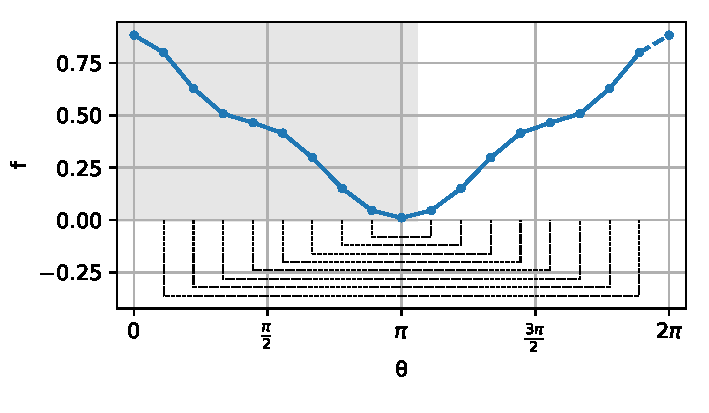
\includegraphics{img/even_parity_demo.pdf}
  \caption{Demo of the reduced integration interval for integrals over an even-parity function.
  The grey area marks those points that are actually included in the discrete summation.
  The dashed lines at the bottom link points of equal value in the full interval
  and their counterparts in the half interval.}
  \label{fig:even_parity_demo}
\end{figure}

Summarizing:
\begin{itemize}
  \item If the normalization factor is $1/n_{\theta,1}$, the inner points need to be weighted by $2$ and only the endpoints of the half-interval are weighted by $1$.
  \item If the normalization factor is $1/(n_{\theta,2}-1)$, the inner points need to be weighted by $1$ and only the endpoints need to be weighted by $1/2$.
\end{itemize}


\FloatBarrier
\newpage
\section{Midpoint vs. Trapezoidal} \label{sec:midpoint_vs_trapz}
The midpoint rule and the trapezoidal rule are used to approximate the one-dimensional integral
of a function~$f$ over a finite interval~$[a,b]$.
The integrand has to be evaluated at the centers of the intervals for the midpoint rule:
\begin{equation}
  A_\mathrm{mid} = \Delta x \left[   f \left(a + \frac{1}{2} \Delta x \right)
                                   + f \left(a + \frac{3}{2} \Delta x \right)
                                   + ...
                                   + f \left(b - \frac{1}{2} \Delta x \right) \right] \, .
\end{equation}
The error estimate for the midpoint rule is:
\begin{equation}
  \left|\int\limits_a^b f(x) \,\mathrm{d}x - A_\mathrm{mid} \right|
  \leq
  \frac{M_2 (b-a)^3}{24 n^2}
\end{equation}
where $M_2$ is the maximum of the absolute value of $f''(x)$ over the interval $[a,b]$.

The integrand has to be evaluated at the borders of the intervals for the trapezoidal rule:
\begin{equation}
  A_\mathrm{trapz} = \Delta x \left[   1/2 f(a)
                                     +     f(a +   \Delta x)
                                     +     f(a + 2 \Delta x)
                                     + ...
                                     +     f(b -   \Delta x)
                                     + 1/2 f(b)\right] \, .
\end{equation}
The error estimate for the trapezoidal rule is:
\begin{equation}
  \left|\int\limits_a^b f(x) \,\mathrm{d}x - A_\mathrm{trapz} \right|
  \leq
  \frac{M_2 (b-a)^3}{12 n^2}
\end{equation}
where $M_2$ is the maximum of the absolute value of $f''(x)$ over the interval $[a,b]$.

This info is quoted from \texttt{https://en.wikipedia.org/wiki/Riemann\_sum}.
